\documentclass{article}
\usepackage{geometry}
\usepackage{listings}
\usepackage{color}
\usepackage{hyperref}
\usepackage{titlesec}
\usepackage{parskip}
\usepackage{sectsty}
\usepackage{pgfplots}
\usepackage{multirow}
\usepackage{float}
\pgfplotsset{compat=1.18}
\definecolor{codebackground}{rgb}{0.95,0.95,0.95}
\definecolor{mygray}{rgb}{0.5,0.5,0.5}

\lstset{
    basicstyle=\ttfamily,
    backgroundcolor=\color{white},
    keywordstyle=\color{blue},
    commentstyle=\color{mygray},
    showstringspaces=false,
    numbers=left,
    numberstyle=\tiny,
    numbersep=5pt,
    breaklines=true,
    frame=single,
    breakatwhitespace=false,
}

\geometry{a4paper, margin=.75in}

\title{\textbf{Operating Systems II \\Spring 2024\\
        Lab Exam
    }}
\author{
    \Large{\textbf{Soham Rajesh Pawar}}\\
    \textbf{CS22BTECH11055}
}

\date{\large{\texttt{April 30, 2024}}}

\begin{document}
\maketitle

\section{Coding Approach}
\textbf{
    The code uses multithreading to get the perfect numbers within a specified range.\\
    Perfect numbers are numbers whose divisors(excluding itself) sum up to the number itself.\\
    Eg. 6, 28, 8128, etc.
}
\subsection{Common Routine:}
\begin{lstlisting}[language=C, caption={Routine 1}, label={code-get-rd}, backgroundcolor=\color{codebackground}]
    void routine(int index)
    {
        for (int i = index; i <= n; i += k)
        {
            if (perfect(i))
            {
                sem_wait(&print);
                outfile << i <<" : Found by thread " << index << "\n";
                sem_post(&print);
                total.fetch_add(1);
            }
        }
    }
\end{lstlisting}
\textbf{
    \begin{enumerate}
        \item{Note that the code contains an atomic int variable \texttt{total} i.e responsible for counting the number of perfect numbers encountered.}
    \item{Each thread processes the numbers that are i modulo k, where i is the index/id of the thread. Note that thread k processes numbers that are 0 modulo k}
    \item{Each thread makes a call for the \texttt{perfect function} which tells them if the number they are currently processing is perfect or not.}
    \item{If yes, then they print their discovery in outFile.txt atomically(to avoid messy printing) and also increment total. Else move on.}
    \end{enumerate}
}
\newpage
\subsection{Function:}
\begin{lstlisting}[language=C, caption={Routine 1}, label={code-get-rd}, backgroundcolor=\color{codebackground}]
    bool perfect(int n)
    {
        int sum = 0;
        for (int i = 1; i < n; i++)
        {
            if (n % i == 0)
                sum += i;
        }
    
        if (sum == n)
            return true;
        else 
            return false;
    }
\end{lstlisting}
\textbf{
    The correctness of the function is obvious.
}

\section{Verification}
\textbf{
    \begin{enumerate}
    \item{Verification can be done by referring to sources which have already performed the said task successfully.}
    \end{enumerate}
}
\section{Output Time Analysis}
\subsection{Total Time vs N:}
\texttt{
    N is in powers of 10, 
    K is 8\\
}
% K	\hspace{1mm} Time taken(s)\\
% 1	\hspace{1mm}0.220093 \\
% 2	\hspace{1mm}0.109615 \\
% 4	\hspace{1mm}0.055748 \\
% 8	\hspace{1mm}0.028887 \\
% 16	\hspace{1mm}0.034837 \\

% \begin{figure}[h]
%     \centering
%     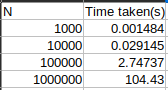
\includegraphics[width=\textwidth]{1.png} % Replace 'your_figure_filename' with the actual filename
%     \label{fig:your_label}
% \end{figure}
\begin{table}[H]
    \centering
    \begin{tabular}{|c|c|}
    \hline
    \textbf{N} & \textbf{Time (seconds)}\\
    \hline
    3 & 0.001484 \\
    \hline
    4 & 0.029145  \\
    \hline
    5 & 2.74737  \\
    \hline
    6 & 104.43 \\
    \hline
    \end{tabular}
    \caption{Execution Times}
    \label{tab:execution_times}
    \end{table}

\subsection{Total Time vs Number of Threads, K:}
\texttt{
    N is 10000\\
}
% \begin{figure}[h]
%     \centering
%     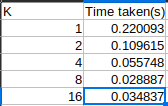
\includegraphics[width=\textwidth]{2.png} % Replace 'your_figure_filename' with the actual filename
%     \label{fig:your_label}
% \end{figure}
\begin{table}[H]
    \centering
    \begin{tabular}{|c|c|}
    \hline
    \textbf{K} & \textbf{Time (seconds)}\\
    \hline
    1 & 0.220093 \\
    \hline
    2 & 0.109615 \\
    \hline
    4 & 0.055748 \\
    \hline
    8 & 0.028887 \\
    \hline
    16 & 0.034837 \\
    \hline
    \end{tabular}
    \caption{Execution Times}
    \label{tab:execution_times}
    \end{table}

\newpage
\end{document}